The results of the experiments using different training sample sizes for the SVM classifiers are displayed in table \ref{tab:svm} and figure \ref{fig:svm}. As more training samples are used to train the SVM classifier performance increases, which is expected for supervised classification. When the training set size reaches more than 75 images per class the classifiers perform worse, possibly due to overfitting on context cues. In the final model, for example, faces that rank high in the airplanes-SVM often have a sky-blue background (see figure \ref{photo:man}), which is also the case for the highest ranked airplanes (see figure \ref{photo:airplane}).
\begin{figure}[H]
\begin{subfigure}[b]{0.5\textwidth}
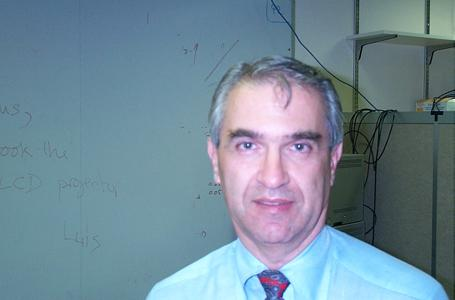
\includegraphics[width=0.5\textwidth]{img003}
\caption{Highest ranked face in the airplane classifier}
\label{photo:man}
\end{subfigure}
\begin{subfigure}[b]{0.5\textwidth}
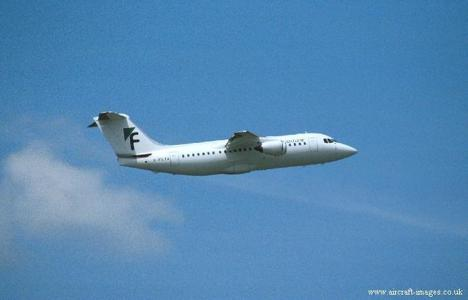
\includegraphics[width=0.5\textwidth]{img010}
\caption{Highest ranked airplane in the airplane classifier}
\label{photo:airplane}
\end{subfigure}
\caption{Images in the final model for the airplane classifier}
\end{figure}
  
\begin{table}[H]
\begin{tabular}{|c|ccccc|}
\hline
\textbf{Training set size} & \textbf{AP Airplanes} & \textbf{AP Cars} & \textbf{AP Faces} & \textbf{AP Motorbikes} & \textbf{MAP}\\
\hline
30 & 0.6647 & 0.8898 & 0.3772 & 0.5184& 0.6125\\
50 & 0.6484 & 0.9096 & 0.8780 & 0.6627 & 0.7747\\
70 & 0.6531 & 0.8441 & 0.7156 & 0.7590 & 0.7429\\
75 & 0.6447 & 0.9053 & 0.9510 & 0.7516 & 0.8132\\
90 & 0.6426 & 0.8697 & 0.5227 & 0.6963 & 0.6828\\
\hline
\end{tabular}
\caption{Effect number of training set size (per class) for SVM, Sift type: dense, Color space: opponent}
\label{tab:svm}
\end{table}

A surprising result is that the airplane and car classifiers obtain a stable performance for the different training set sizes. This is clearly shown in Figure \ref{fig:svm}. A possible explanation is that the airplane and car images have little noise (which can cause overfitting of the model) and do not require a lot of training data to be modeled. The images in the dataset for each of these classes are taken from the same angle and the form of the objects are more similar than faces or motorbikes, which result in a more stable performance.

\begin{figure}[H]
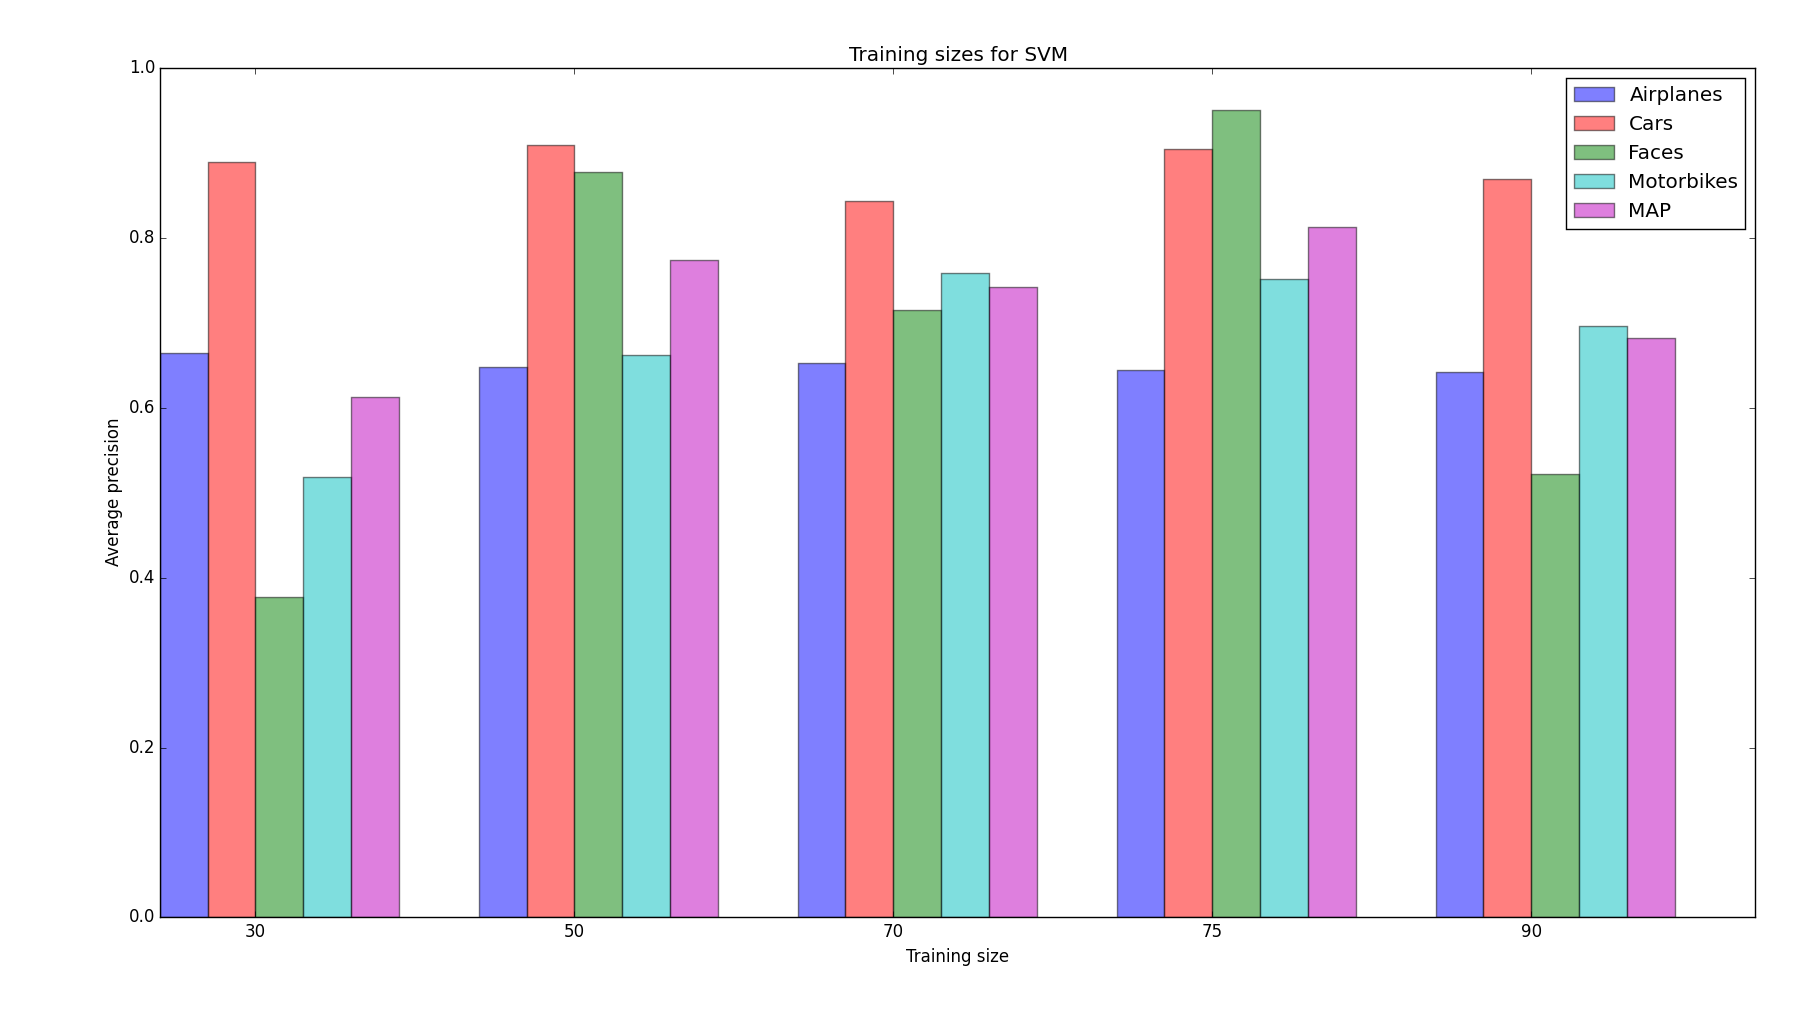
\includegraphics[width=\textwidth]{../plots/training_size_SVM}
\caption{Effect of training size for SVMs on AP}
\label{fig:svm}
\end{figure}
